% !TEX root = ../../main.tex
% !TEX spellcheck = en_GB

\section{Analysis}
In contrast to the pure sine, the C-major consists of several frequencies, as shown in \cref{fig:fftc4}.

\begin{figure}
	\centering
	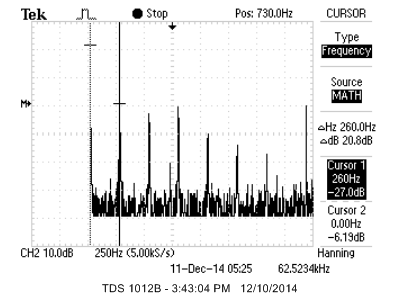
\includegraphics[width=0.7\linewidth]{gfx/fft_C4.jpg}
	\caption{Frequency spectrum of C$_4$ played on a piano \cite{fft_c4}.}
	\label{fig:fftc4}
\end{figure}

These frequencies are evenly spaced, and the solutions presented in \cref{sec:simpleanal} are still valid to use.
Here the solution of changing the sampling frequency is still not valid due to limitations on the Blackfin, and the primary target of the analysis is if it is possible to use the same approach as in the pure sine implementation: Creating a new tone at the target frequency.

The approach again focuses on the steps
\begin{enumerate}
	\item Find the input tone.
	\item Create new tone at target frequency.
	\item Play output tone.
\end{enumerate}

\paragraph{Finding the input tone}
In the sine part, the frequency was found using Instantaneous Frequency.
This approach may still be valid, but would require the ratio between the fundamental and every harmonic frequency to be exactly the same each time.
Should the ratios for the fundamental and the first to harmonics be e.g. 3, 2 and 1, the output of the Instantaneous Frequency would be as shown in \cref{tab:CmajorIF}.

\begin{table}
	\centering
	\begin{tabular}{l c}
		\toprule
		Note & IF \\
		\midrule
		C$_4$ & \num{436.043} \\
		D$_4$ & \num{489.442} \\
		E$_4$ & \num{549.380} \\
		F$_4$ & \num{582.047} \\
		G$_4$ & \num{653.325} \\
		A$_4$ & \num{733.333} \\
		B$_4$ & \num{823.138} \\
		\bottomrule
	\end{tabular}
	\caption{IF values if including the first two harmonic frequencies.}
	\label{tab:CmajorIF}
\end{table}

Another approach could be to use FFT to determine the tallest peak, leading to a not very accurate measurement, approximately \SI{\pm50}{\hertz}, bandpass filter this frequency bin, removing everything else, and the calculate the Instantaneous Frequency.
The found frequency can then be compared to a table of the C-major frequencies and their harmonics, allowing the tone to be determined.
Then the new pitch shifted tone can be created with a number of harmonics.